\section{How to Collect Data}



\subsection{ Data sources}
    \begin{itemize}
    \item
	- usage data from tools of course
\item
	- usage data in user study smaller setting is augmented by user explicit feedback to establish ground truth (e.g. search result was good) 
\item
	- smaller studies can ask questions about user activities that add rationale to the usage data that tells why user is doing what they are doing
\item 
	- small studies can generate a metric you can use with larger data source that does not have augmented data.  E.g. structured navigation that Robillard did supports a larger study such as what we did at ABB.
    \end{itemize}

\subsection{ Building Data Collection} 
  \label{BuildingDataCollection}

	Tailoring usage data collection to specific needs helps optimize the volume of data and privacy concerns when collecting information from software development applications.  While a general solutions described in the next sections collect all events from the Integrated Development Environment (IDE), limiting the data collection to specific areas for research can improve the result.  A process for defining the desired data can follow structures such as Goal-Question-Metric \cite{basili-GQM}  that refines a high-level goal into specific metrics to generate from data.  For example, to study the navigation practices of developers, we perfrom the GQM process as follows:
    \begin{itemize}
\item 
	Goal
\subitem 
	To assess and compare the use of structured navigation by developers in our study
\item 
	Possible Question(s)
\subitem
	What is the frequency  of navigation commands developers use when modifying source code?
\subitem
	What portion of navigation commands developers use are structured navigation rather than unstructured navigation?
\item
	Metric
\subitem
	Navigation Ratio is the proportion of the number of structured navigation commands used to the number of unstructured navigation commands used by a developer in a given time period (e.g. a day)

	    \end{itemize}

The next step is selecting the data to collect from the IDE related to the Metric defined for Navigation Ratio.  For this we identify the  commands related to structured navigation (in Visual Studio) as follows:
\begin{itemize}
\item 
 Navigate To (Ctrl+,) is a fuzzy search interface that lists identifiers matching the selected string 
\item Go To Definition (F12) brings up the code that defines the selected identifier 
\item View Call Hierarchy (Ctrl+K Ctrl+T) provides a two way analysis of an identifier's dependencies and uses
\item Class View (Ctrl+W, C) provides a browser and search function for classes and class hierarchy
\item Find All References (Ctrl+K,R) provides a list of lines that reference an identifier
\item Navigate to Event Handler in the XAML editor shows the event handler for an object
\item View Class Diagram generates a class diagram 
\item View Object Browser is a search tool and browser
\end{itemize}

Next we identify the commands related to unstrctured navigation as follows:
\begin{itemize}
\item selecting a file in an explorer window
\item selecting the tab for a file
\item using arrow and page up/down keys to go up/down through a file
\item scrolling, 
\item clicking on a file element
\item using GoTo Line command
\item using Find In Files command
\item using Quick Find command
\end{itemize}

These identified commands form the set of actions that usage data needs to collect to calculate the navigation ratio metric.  Notice that the commands are a mixture of defined actions within the tool and actions that result from mouse actions such as selecting a window or a window tab.  The latter need further refinement to determine how the usage monitor can identify these actions from available events in the IDE.  This is discussed in further detail in section \ref{buildItYourself}.

Assessing commands within a time duration (e.g. day) requires that we collect a time-stamp for each command.  Simply using the time as a "by variable" where we stratify data according to time is a straight-forward conversion.  The time-stamp can be converted to a date allowing data to be grouped by the day of the events.  Similarly the time-stamp can be convered to hour to look at events each hour of any given day.
Calculating duration or elapsed time for a command or set of commands adds new requirements to monitoring.  Specifically, the need to collect events that relate to when the application or IDE is being used and when it is not and the need to collect additional events that occur when the user has moved on from the command of interest.  This is discussed in further detail in section \ref{buildItYourself}.

Concerns over privacy intrusion makes usage monitoring a flash point for some people.  Privacy concerns can be divided into concerns about what data is collected that may expose the user or parts of the source code to prying eyes and who the data and aggregates of it are shared with.  

To alleviate concerns about what data is collected, steps such as hashing sensitive pieces of information can reduce the concern. If you collect information like window titles they can contain filenames, web site titles, or even email titles.  Hashing these names provides a measure of assurance that the data are less easily identifiable with the user of the system and with sensitive subjects they may be working on.   Collecting a user identification makes this data very helpful for understanding distribution of practices, however, this makes it more sensitive as well.  Generating an anonymous identifier to identify distinct users helps alleviate the concern that data will be associated with the user.

To reduce concerns about who the data are shared with, create a statement of policy around this.  If the data is for research purposes only, you can state specifically whom will have access to the data and what they will do with it.  Limiting statements such as not reporting data at the individual level helps this policy reduce concerns about who the data is shared with.


    \begin{itemize}
\item
      What data is relevant to collect? (data granularity depends on needs of subsequent analysis and anticipated space and time overhead; collecting aggregate data vs. individual events; mention that data should be timestamped as a lot of subsequent analyses depend on that)
    \item
      How to modify existing tools to collect data? (events are a good communication paradigm; centralizing the logger in the code allows for consistent log messages and easy maintenance; trade-offs in storing logs as highly structured or somewhat unstructured data)
    \item
      Privacy and anonymity considerations when collecting data. (what not to collect, using hashes to protect user identities)
      
     
    \item
    	Existing usage data (Mylyn's 99 developers, UDC, etc). %Emerson 
     
    \end{itemize}

\subsection{Instrumenting the IDE -- Using an Existing Framework} %Emerson
  
\begin{enumerate}
	\item 
	There are many existing frameworks to use. We suggest picking on and building off one. (Note: Clone these on github? include packaged with IDE?)
	
	\item Eclipse: Mylyn Monitor. Format: What it was originally intended to be used for. What data it collects. Where to get it. How to install it (w/version info). Example output. Deployment(?)
	
	\item CodingSpectator %https://github.com/vazexqi/CodingSpectator	
	
	\item Hackystat\cite{V:johnson2003beyond}, %https://code.google.com/p/hackystat/

	\item Zorro\cite{Kou2010Operational}. %same as Hackystat? How about VS tool?
	
	\item CodeAlike has one, too, but they get the data!
	
	\item Romain Robbes -- maybe for Visual Studio, but for smalltalk? SHould be in chapter.
\end{enumerate}

\subsection{Instrumenting the IDE -- Building it Yourself for Visual Studio} 
\label{buildItYourself}

This section is a tutorial sequence of exercises that support student projects for implemeting a personal monitoring tool for Visual Studio.  Each exercise allows the student to discover technical aspects of monitorning tools in a way that builds capabilities towards a monitoring tool.  Readers attempting the tutorial should be familiar with the .NET event model used to manage GUI commands in .NET applications, have demonstrated capability programming in C sharp, and have working knowledge of Visual Studio.  

The goal is to build a Visual Studio Extension that collects key command events from Visual Studio that generate the Navigation Ratio metric (See \ref{BuildingDataCollection} for each day's development activity.  The extension will startup when Visual Studio starts, automatically collect events from the IDE, and save the data to a local file.  For simplicity, the extension will not perform any background processing thus the user may notice a delay on Visual Studio startup due to this exension's setup process.  The first time the extension runs, it will create a configuration file that allows the user to specifiy which events it will record and how it will classify those events as structured or unstructured navigation.  The extension will create a new time-stamped log file each time it starts and record the events for that execution of Visual Studio in the log file. 


 \begin{Exercise}[type={program}, difficulty={1}]
\begin{enumerate}
\item
The first step in instrumenting Visual Stuidio is to create a Visual Studio Extension that creates a log file when it starts.   Microsoft provides a project creation wizard for generating a Visual Stuido extension (called a Package) when you install the Visual Studio SDK.  So first install the Visual Studio SDK.  

\item Create a new project in C sharp selecting Extensibility and Visual Studio Package under the new project creation dialog as shown in figure \ref{fig:ProjectCreation}.  
\begin{figure}[h]
	\centering
	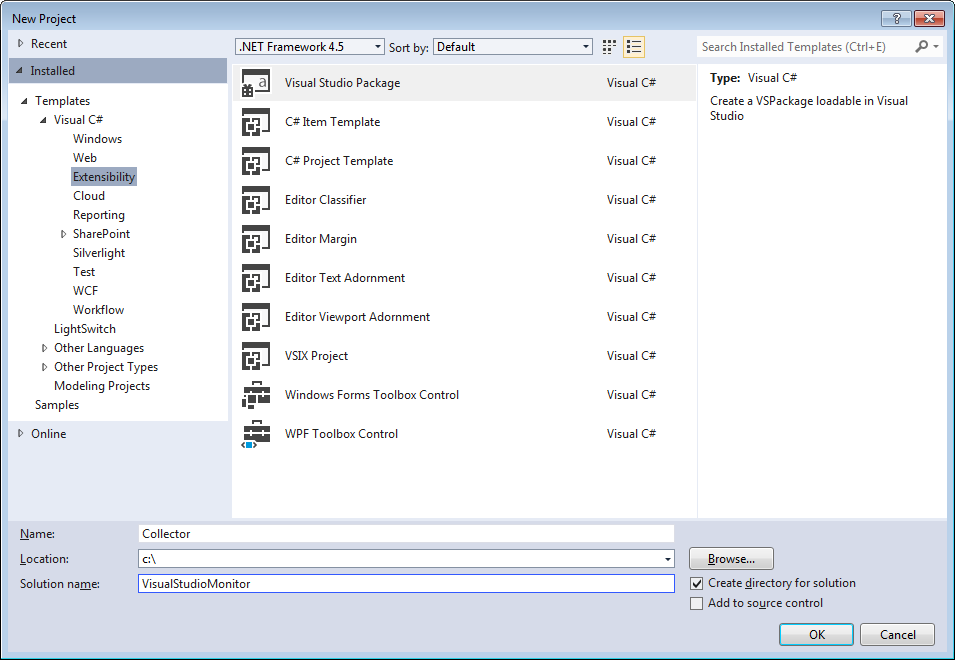
\includegraphics[width=4in]{Graphics/CreateVSIXExtension.png}
	\caption{Create a Visual Studio Extension}
	\label{fig:ProjectCreation}
\end{figure}

Give the project and solution a name and follow the default options for each step of the wizard.  When asked to specify what type of extension, click only the option to generate a menu command.  In the following step, give the menu command a name of "Stop Monitoring" and a command ID of "StopCollector".  This menu option will allow the user to halt collection of data if they wish without quitting Visual Studio.  
\end{enumerate}
\end{Exercise}

 \begin{Answer}

\begin{enumerate}
\item
After creating the project and solution, the solution explorer should look like figure \ref{fig:SolutionExplorer} showing the project files necessary for the extension to work.
\begin{figure}[h]
	\centering
	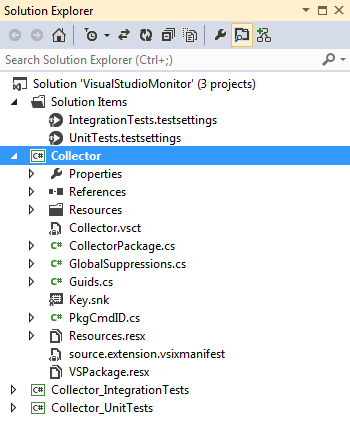
\includegraphics{Graphics/SolutionExplorer.png}
	\caption{Solution Explorer with Visual Studio Extension}
	\label{fig:SolutionExplorer}
\end{figure}
\end{enumerate}
\end{Answer}

\begin{Exercise}[type={program}, difficulty={1}]
\begin{enumerate}
\item
Good practice in extension development is to create a separate project (dll) for logic specific to the extension.  Add a class library type project to  the "Monitor" solution provide the data collection from Visual Studio and call it "Monitor".
\item
The next step is to create a static class that will manage the log file including starting, stoping recording data, and inserting data into the log file.  We will call this class "DataRecorder".   
Create a "DataRecorder" Class in the Collector project.  Becase we don't want more than one recorder running at a time and want to access this class without instantiating it, make the class static.  Have the DataRecorder write a message to the file whenever it starts and stops.
\item
Finally, insert a call to DataMonitor.Start() at the end of the Initialize() method in the CollectorPackage class.  This will start the monitoring each time Visual Studio starts.  You will need to add a reference for the "Monitor" project to the Collector project, sign the Monitor project (you can use the snk file generated when the solution was created in step 1), then rebuild the solution.
\end{enumerate}
\end{Exercise}

\lstset{language=Java,
captionpos=b,
tabsize=3,
frame=lines,
numbers=left,
numberstyle=\tiny,
numbersep=5pt,
breaklines=true,
showstringspaces=false,
basicstyle=\footnotesize,
emph={label}}

\begin{Answer}

The call to DataRecorder.Start() is inserted in the CollectorPackage as shown in Listing \ref{code:StartCall}.
\begin{lstlisting}[caption=Call to DataRecorder.Start(),label=code:StartCall,float=h]
        /////////////////////////////////////////////////////////////////////////////
        // Overridden Package Implementation
        #region Package Members

        /// <summary>
        /// Initialization of the package; this method is called right after the package is sited, so this is the place
        /// where you can put all the initialization code that rely on services provided by VisualStudio.
        /// </summary>
        protected override void Initialize()
        {
            Debug.WriteLine (string.Format(CultureInfo.CurrentCulture, "Entering Initialize() of: {0}", this.ToString()));
            base.Initialize();

            // Add our command handlers for menu (commands must exist in the .vsct file)
            OleMenuCommandService mcs = GetService(typeof(IMenuCommandService)) as OleMenuCommandService;
            if ( null != mcs )
            {
                // Create the command for the menu item.
                CommandID menuCommandID = new CommandID(GuidList.guidCollectorCmdSet, (int)PkgCmdIDList.StopCollector);
                MenuCommand menuItem = new MenuCommand(MenuItemCallback, menuCommandID );
                mcs.AddCommand( menuItem );
            }
            DataRecorder.Start();
        }
        #endregion
\end{lstlisting}

The source code for the DataRecorder.cs file is shown in Listing \ref{code:DataRecorder}
\begin{lstlisting}[caption=Data Recorder Class,
  label=code:DataRecorder,
  float=h]
using System;
using System.Collections.Generic;
using System.Linq;
using System.Text;
using System.Threading.Tasks;

namespace Monitor
{
    public static class DataRecorder
    {
        public static void Start() {
            logDirectoryPath = System.IO.Path.GetTempPath();
            logFileName = System.IO.Path.Combine(logDirectoryPath, "collector " + DateTime.Now.ToString("yyyy-MM-dd HH.mm.ss") + ".log");
            try {
                using (System.IO.StreamWriter streamWriter = new System.IO.StreamWriter(
                    new System.IO.FileStream(logFileName, System.IO.FileMode.OpenOrCreate, System.IO.FileAccess.Write, System.IO.FileShare.ReadWrite)
                    ))
                {
                    streamWriter.WriteLine("Collector Started");
                }
            } 
            catch (System.IO.IOException ioexception) {
                Console.WriteLine("Error creating log file "+ioexception);
            }
         }

        public static void Stop() {

                WriteLog("Collector Stopped");
            
        
        }

        public static void WriteLog(string logToWrite)
        {
            try
            {
                using (System.IO.StreamWriter streamWriter = new System.IO.StreamWriter(
                    new System.IO.FileStream(logFileName, System.IO.FileMode.Append, System.IO.FileAccess.Write, System.IO.FileShare.ReadWrite)
                    ))
                {
                    streamWriter.WriteLine(logToWrite);
                }
            }
            catch (System.IO.IOException ioexception)
            {
                Console.WriteLine("Error writing to log file " + ioexception);
            }
        
        }

        private static string logFileName;
        private static string logDirectoryPath;
    }
}

\end{lstlisting}
\end{Answer}

 \begin{Exercise}[ type={program}, difficulty={1}]
Visual Studio processes all command events through the DTE object that also provides the API for extending Visual Studio.  Command events are any command that the user performs in the IDE using a menu, shortcut button, or quick launch command.  Each command in Visual Studio has a GUID identifier and an integer number that together make it distinct.  The commands also have a text name usually representing a position in the menu structure where the command lives.

Fortunately the DTE object has a query method that lists all the commands it manages.  This interface will query Visual Studio for all the supported commands in the IDE.  There are several versions of the DTE object corresponding to versions of Visual Studio.  Depending on the commands of interest, each version may need to be queried for its commands.  

In this step, build the classes required to query the DTE for all commands and store them for later use preferably in a text or XML format file.  You will need an extra field to allow you to select or classify the command to be monitored.  In the next step we will read in the file and regester an event handler for each command that we wish to monitor.  Call the method(s) to query and store from the Start() method from the DataRecorder class in the previous exercise so that the Monitor will save the commands on startup.

Recommended design pattern for this exercise is a Simple Factory pattern.  With this pattern an abstract base class provides common definitions for class fields that will be used for monitoring different Visual Studio events, conversion of those fields to and from the storage format, and (eventually) calling the WriteLine method in the recorder when the event fires.  The concrete creator class is the class specific to Visual Studio commands that manages the fields available from the DTE.Command class.  The client in the Simple Factory pattern is a class that maintains the collection of events that either gets read from the file or queried from Visual Studio.
\end{Exercise}

\begin{Answer}
The previous exercise adds a feature to query the DTE and save the commands to a file.  The instruction hinted that more than one class may be used, though the implementation could take place without class members that hold the DTE Command attributes.  The following class design provides the ability to store and retrieve command attributes and anticipates other types of monitored events outside the scope of commands.

The AbstractMonitoredEvent class in listing %\ref{code:AbstractMonitoredEvent}
 provides an abstraction of what data and methods are needed to setup event monitoring in VisualStudio.  Initally the class only deals with data that we save about the event, later it will include methods and parameters used to register the event and capture its invocation.

%\lstinputlisting[caption=Abstract Monitored Event, label=code:AbstractMonitoredEvent,   float=h]{c:/VisualStudioMonitor/Monitor/AbstractMonitoredEvent.cs}

The MonitoredCommandEvent in listing %\ref{code:MonitoredCommandEvent}
makes the AbstractMonitoredEvent class concrete for Visual Studio commands.  It implements a constructor that builds a MonitoredCommandEvent object from the Command class of the DTE or a constructor that builds from an XElement.  An output method ToXElement translates the object to XML for saving.
%\lstinputlisting[caption=MonitoredCommandEvent,  label=code:MonitoredCommandEvent,  float=h]{c:/VisualStudioMonitor/Monitor/MonitoredCommandEvent.cs}

The MonitoredEventFactory in listing %\ref{code:MonitoredEventFactory}
 is a static class that completes our Simple Abstract Factory pattern provding the methods to create an object inheriting from AbstractMonitoredEvent from an XElement or a Command object.  
%\lstinputlisting[caption=MonitoredEventFactory,  label=code:MonitoredEventFactory,  float=h]{c:/VisualStudioMonitor/Monitor/MonitoredEventFactory.cs}

The MonitoredEventCollection in listing %ref{code:MonitoredEventCollection}
 is the Client in our pattern that maintains a "stock" of all the monitored events we need to manage.  It currently provides methods to read MonitoredEvents from a file, save them to a file, and query them from the Visual Studio DTE.  Events are managed in a List object belonging to this class.   The constructor initializes the List object from a configuration file if the file exists, otherwise it initializes the List object from the Visual Studio DTE's Command object and saves the List to the configuration file. 
%\lstinputlisting[caption=MonitoredEventCollection,  label=code:MonitoredEventCollection,  float=h]{c:/VisualStudioMonitor/Monitor/MonitoredEventCollection.cs}

\end{Answer}

\begin{Exercise}
The previous exercise adds a feature to query the DTE and save the commands to a file.  In this step we will add the ability to read that file and register event processing to save a log when each command we wish to monitor is used in the IDE.  
\end{Exercise}
 summary:
\begin{enumerate}
	\item 
	Identify the goal (or research questions) and metrics for measurement that requires IDE data.  express attributes of the goal such as how time should be measured, how events should be classified or grouped, and derived calculations.
	\item
	Identifying  IDE API interfaces necessary to accomplish the measurement goal.  Examples window showing events, scrolling in the editor, clicking on code lines, Command events, automated events (e.g. build begin and end).
	\item
	The event interceptor model, intercepting IDE events transparently to the user.  consider Throttling the capture of near real-time events such as scrolling.
	\item
	Considerations for anonymizing the collected data
	\item
	IDE data collection tooling.  Build tooling for ease of use and installation.  Planning logging interface for offline and online data collection.  Handling data store access.  Ways to address security.  
	\item
	End user communication including anonymity, statement of intended use, restrictions on use, optional participation
	
\end{enumerate}
- detailed how to walkthrough 

\subsection{Eclipse Usage Data Collector}

This section outlines how to collect IDE usage data using Eclipse's Usage Data 
Collector (UDC).\footnote{\url{http://www.eclipse.org/epp/usagedata/}}
The UDC framework was originally build by the Eclipse Foundation, as a way to measure how the 
community was using the Eclipse IDE.
While UDC was included in official Eclipse releases and data was collected from
hundreds of thousands of Eclipse users between 2008 and 2011, the project was eventually shut down, 
and UDC was removed from official Eclipse releases.
However, the source code for UDC remains available and researchers can still use and deploy it.

\subsubsection{What Data is Collected}

The Eclipse Data Collector records the following types of Eclipse information:

\begin{itemize}
 
\item The runtime environment, such as the operating system and Java Virtual Machine.

\item Environment data, such as which bundles are loaded and when Eclipse
starts up and shuts down

\item Actions and commands that are executed, via menus, buttons, toolbars, and hotkeys.

\item Views, editors, and perspectives that are invoked.

\end{itemize}

\noindent
Let's look at an example of an event that UDC produces on a developer's machine:
\vspace{4mm}

\noindent
\begin{small}
\begin{tabular}{llllll}
\textbf{what}&\textbf{kind}&\textbf{bundleId}&\textbf{bundleVersion}&\textbf{description}&\textbf{time}\\
\hline
executed&command&org.eclipse.ui&3.7.0.v20110928-1505&org.eclipse.ui.edit.paste&1389111843130\\
\end{tabular}
\end{small}

\vspace{4mm}
\noindent
The first column tells us what kind of thing happened -- in this case, something was executed.
The second column tells us what was executed -- in this case, a command.
The third column tells us what bundle this event belonged to -- in this case, Eclipse's user interface bundle.
The fourth column gives us the version of the bundle.
The fifth tells us the name of the command that was executed -- in this case, paste.
The final column tells us when the command was executed, in Greenwich Mean Time -- in this case, January 7th, 2014 at 16:24:03 GMT.


\subsubsection{Limitations}

Apart from general limitations of collecting usage data (Section~\ref{sec:limitations}),
one significant limitation of UDC that we have found is that sometimes it has 
unexpectedly incomplete data.
For example, in planning for a study involving when people ran their JUnit tests,
we found that UDC recorded an event when the ``Run \textgreater~Run As \textgreater~Run as JUnit Test'' menu item was selected,
but not when the ``Run As'' button was pressed on the toolbar.
We suspect that the reason has to do with how different user interface accordances
invoke the same functionality.
In general, when you are planning on running a study with UDC, be sure to know what 
types of events you are looking for, and test them to make sure UDC captures those events.

\subsubsection{How to Use It}

Collecting data for your own research is fairly straightforward with Eclipse UDC,
and we describe how to do so here.
We also include an accompanying screencast that shows the 
basics.\footnote{\url{https://docs.google.com/file/d/0B7DV-T4_2mpKRWgwRnJnTWpvN0E/edit}}
%TODO move this screencast to youtube, once you're happy

\paragraph{Gathering Data Using the UDC Client.}

Let's talk about how data is collected on a developer's machine.
Since UDC was last included in the Eclipse Indigo SR2 
release,\footnote{(\url{http://www.eclipse.org/downloads/packages/release/indigo/sr2}}
if you have the option of which Eclipse to use, we recommend downloading
that version.
By default, UDC starts collecting data when Eclipse is start up. 
You can verify this by going to ``Windows \textgreater~Preferences'', then
select the ``Usage Data Collector'' item (Figure~\ref{fig:prefPage1}).
The \textit{Enable capture} option should be checked.

\begin{figure}
  \centering
  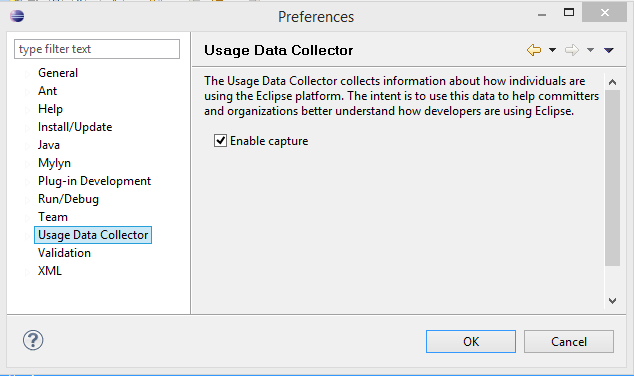
\includegraphics[scale=.58]{prefPage1}
  \caption{Eclipse Usage Data Collector preference page.}\label{fig:prefPage1}
\end{figure}

Before looking at the data, execute a few commands and open a few views 
in Eclipse.
Then, on your file system, open the following path as a subdirectory
of your current workspace (Figure~\ref{fig:filesystem}): 

\vspace{4mm}
\texttt{.metadata/.plugins/org.eclipse.epp.usagedata.recording}
\vspace{4mm}

\noindent
In that folder, depending on how many UDC events have been gathered,
a number of comma separated value (CSV) files will appear, where \texttt{upload0.csv} is the oldest
and \texttt{usagedata.csv} is the newest.
Open up \texttt{usagedata.csv} -- you should notice a large number and a variety of events.
Be sure to look specifically for events that you executed and views that you opened earlier.

\begin{figure}
  \centering
  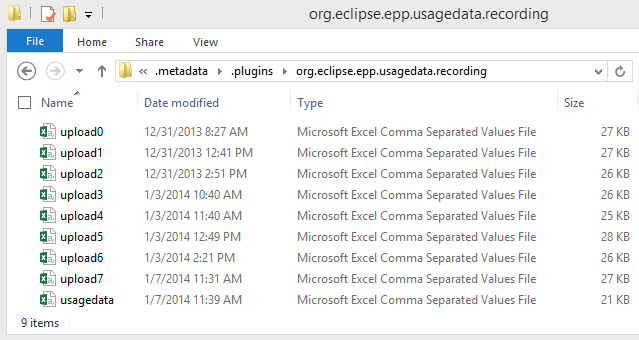
\includegraphics[scale=.58]{filesystem}
  \caption{UDC data files.}\label{fig:filesystem}
\end{figure}

Before doing a study, be aware that Eclipse will ask and periodically attempt to upload
data to the Eclipse foundation server.
You should \emph{not} allow it to do this, because each time data is uploaded, the underlying
CSV files are deleted.
Furthermore, because the UDC project is no longer officially supported, the official Eclipse
UDC server no longer accepts the data, so your usage data is, in effect, lost permanently.
Unfortunately, there is no easy way to tell the UDC client to permanently store
usage data.
An easy workaround is to increase the upload period to 90 days (Figure~\ref{fig:upload}),
which should be enough time to complete the experiment.
The long-term fix for this issue is to modify the source code, as we will explain
how to do shortly, to never upload data.

\begin{figure}
  \centering
  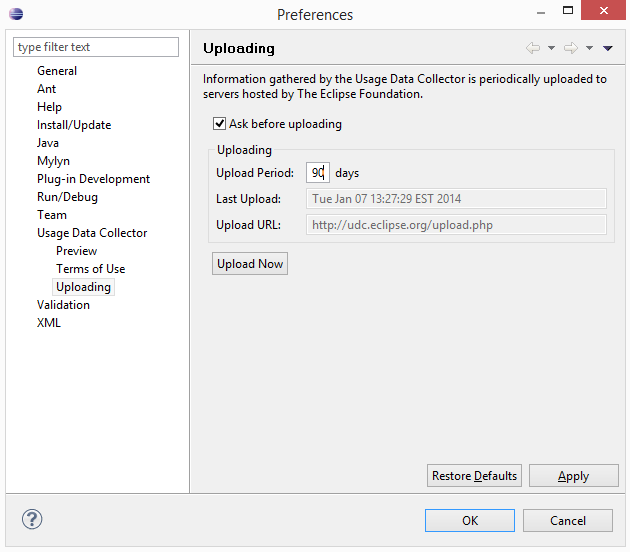
\includegraphics[scale=.58]{upload}
  \caption{Changing the UDC upload frequency.}\label{fig:upload}
\end{figure}

If you're doing a lab experiment, collecting data should be simply a matter of 
copying and deleting the CSV files after each participant has done the experiment.
You can append the files together or put them in a database for analysis.

\paragraph{Modifying the UDC Client.}

You may wish to modify the UDC client yourself, perhaps to add a custom filter for events
or to disable data uploading.
Whatever the reason, making modifications to the client is fairly easy.

The first step is to check out the UDC source code into your Eclipse
workspace using git.\footnote{\url{http://git-scm.com/}}
Here we will again use Eclipse Indigo SR2, but we will specifically be using the 
``Eclipse for RCP and RAP Developers'' download package because we will
modify Eclipse plugins.
Before importing the necessary plugins, we recommend switching to 
the Indigo SR2 tag, to assure compatibility with
Eclipse.
To do so, clone the git repository\footnote{\url{http://git.eclipse.org/c/epp/org.eclipse.epp.usagedata.git/}} 
locally, open up ``Tags'', right click on ``Indigo SR 2'',
then choose ``Checkout''.

To import the projects into Eclipse, right click on the repository, then click 
``Import Projects,'' then ``Import Existing Projects.''
The three core projects to import are:

\begin{itemize}
\item org.eclipse.epp.usagedata.internal.gathering
\item org.eclipse.epp.usagedata.internal.recording
\item org.eclipse.epp.usagedata.internal.ui
\end{itemize}

Next, we recommend a quick smoke test to determine whether you 
can actually make changes to the UDC client.
Open \texttt{UsageDataRecordingSettings.java}, then modify the value of \texttt{UPLOAD\_URL\_DEFAULT}
to \texttt{"my\_changed\_server"}.
Then, create a new debug configuration that is an Eclipse Application, and press 
``Debug'' (Figure~\ref{fig:debugconfig}).
Finally, you can verify that your change worked by going to UDC's Uploading 
preference page, noticing that the Upload URL is now ``my\_changed\_server''.

\begin{figure}
  \centering
  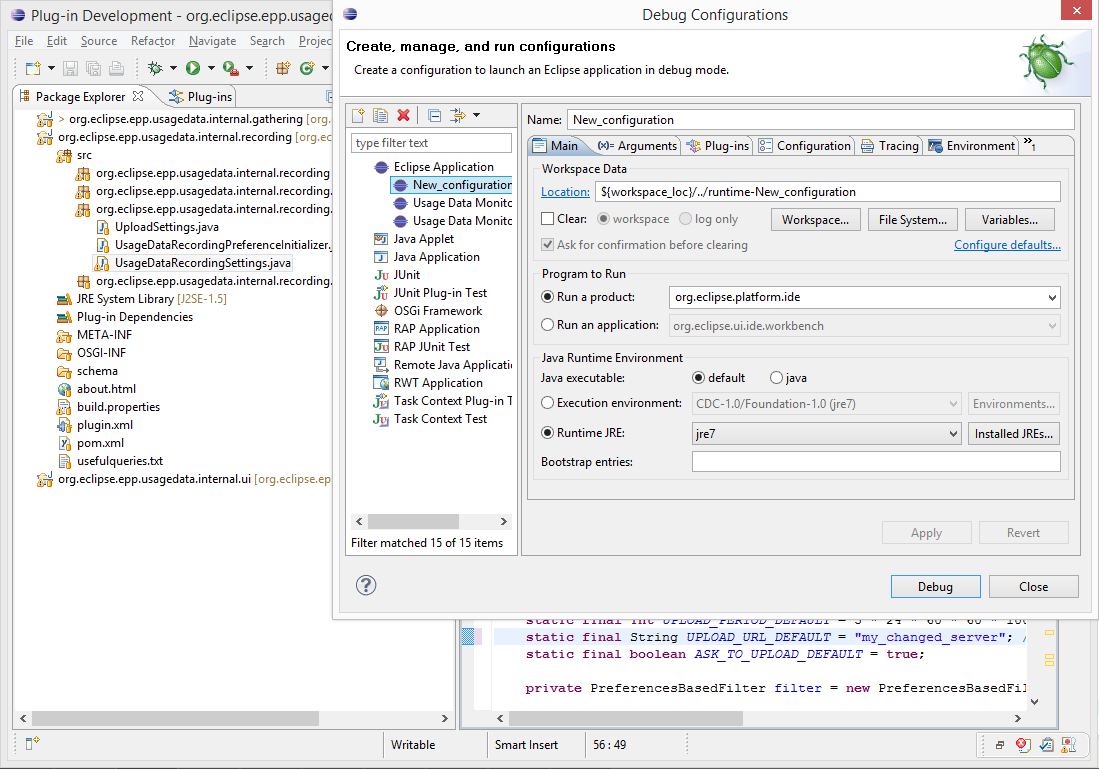
\includegraphics[scale=.58]{debugconfig}
  \caption{Debugging the UDC client.}\label{fig:debugconfig}
\end{figure}

From here, you can make any changes to the UDC client that you wish.
One thing you may want to do is upgrade UDC to work with more recent versions
of Eclipse.
The code is likely currently out of date
because it has not been maintained since the UDC project was shut down.
Another thing you may wish to do is deploy your new version of UDC via
an Eclipse update site to the developers you want to study.
There are many resources on the web for plugin deployment instructions,
such as Lars Vogel's tutorial on creating 
plugins.\footnote{\url{http://www.vogella.com/tutorials/EclipsePlugIn/article.html#deployplugin_tutorial}}

\paragraph{Transmitting Data over the Internet.}

If you do not plan on doing a lab study where you can manually collect UDC usage
files, you will want to have the UDC client send the data to you directly.
As we mentioned, the best way to do this is probably by changing the default
server URL in the client source code.
An easy way to change the server when debugging is by adding the following Java
virtual machine arguments:

\vspace{4mm}
\texttt{-Dorg.eclipse.epp.usagedata.recording.upload-url=http://localhost:8080}
\vspace{4mm}

\noindent
However, simply changing the client to point at a new URL is insufficient, 
because there actually has to be a working server at that URL, ready to 
receive UDC data.
While the source code of official Eclipse server was not officially made 
available, Wayne Beaton from the Eclipse Foundation unofficially released
some of the PHP code from the Eclipse Foundation's server.
If you would like to download that code, you will find it in our git repository.
%TODO need to put this code into git
However, our PHP skills are very basic and we were not immediately able
to get the server working as expected, but we expect that anyone familiar with
debugging PHP should be able to.

\newpage

Creating your own server that receives UDC data is fairly straightforward.
Let's create a simple one using Apache's HttpComponents library,
the same library that UDC uses to upload data.
Specifically, we can create a server by simply extending Apache's tutorial
web server.\footnote{\url{http://hc.apache.org/httpcomponents-core-ga/httpcore/examples/org/apache/http/examples/ElementalHttpServer.java}}
First, we'll need a generic request handler to wait for HTTP connections:

\begin{lstlisting}
import java.io.IOException;
import org.apache.http.ConnectionClosedException;
import org.apache.http.HttpException;
import org.apache.http.HttpServerConnection;
import org.apache.http.protocol.BasicHttpContext;
import org.apache.http.protocol.HttpContext;
import org.apache.http.protocol.HttpService;

/**
 * Based on
 * http://hc.apache.org/httpcomponents-core-ga/httpcore/examples/org/apache
 * /http/examples/ElementalHttpServer.java
 */
class WorkerThread extends Thread {

	private final HttpService httpservice;
	private final HttpServerConnection conn;

	public WorkerThread(final HttpService httpservice, final HttpServerConnection conn) {
		super();
		this.httpservice = httpservice;
		this.conn = conn;
	}

	@Override
	public void run() {
		System.out.println("New connection thread");
		HttpContext context = new BasicHttpContext(null);
		try {
			while (!Thread.interrupted() && this.conn.isOpen()) {
				this.httpservice.handleRequest(this.conn, context);
			}
		} catch (ConnectionClosedException ex) {
			System.err.println("Client closed connection");
		} catch (IOException ex) {
			System.err.println("I/O error: " + ex.getMessage());
		} catch (HttpException ex) {
			System.err.println("Unrecoverable HTTP protocol violation: " + ex.getMessage());
		} finally {
			try {
				this.conn.shutdown();
			} catch (IOException ignore) {
			}
		}
	}
}
\end{lstlisting}

\newpage
\noindent
We'll also need a generic request listener:

\begin{lstlisting}
import java.io.IOException;
import java.io.InterruptedIOException;
import java.net.ServerSocket;
import java.net.Socket;

import org.apache.http.HttpConnectionFactory;
import org.apache.http.HttpServerConnection;
import org.apache.http.impl.DefaultBHttpServerConnection;
import org.apache.http.impl.DefaultBHttpServerConnectionFactory;
import org.apache.http.protocol.HttpService;

/**
 * Based on
 * http://hc.apache.org/httpcomponents-core-ga/httpcore/examples/org/apache
 * /http/examples/ElementalHttpServer.java
 */
class RequestListenerThread extends Thread {

	private final HttpConnectionFactory<DefaultBHttpServerConnection> connFactory;
	private final ServerSocket serversocket;
	private final HttpService httpService;

	public RequestListenerThread(final int port, final HttpService httpService)
			throws IOException {
		this.connFactory = DefaultBHttpServerConnectionFactory.INSTANCE;
		this.serversocket = new ServerSocket(port);
		this.httpService = httpService;
	}

	@Override
	public void run() {
		System.out.println("Listening on port " + this.serversocket.getLocalPort());
		while (!Thread.interrupted()) {
			try {
				// Set up HTTP connection
				Socket socket = this.serversocket.accept();
				System.out.println("Incoming connection from" + socket.getInetAddress());
				HttpServerConnection conn = this.connFactory.createConnection(socket);

				// Start worker thread
				Thread t = new WorkerThread(this.httpService, conn);
				t.setDaemon(true);
				t.start();
			} catch (InterruptedIOException ex) {
				break;
			} catch (IOException e) {
				System.err.println("I/O error initialising connection thread: " + e.getMessage());
				break;
			}
		}
	}
}
\end{lstlisting}

\newpage
\noindent
And finally, the guts of our server:

\begin{lstlisting}
import java.io.IOException;
import org.apache.http.HttpEntityEnclosingRequest;
import org.apache.http.HttpException;
import org.apache.http.HttpRequest;
import org.apache.http.HttpResponse;
import org.apache.http.protocol.HttpContext;
import org.apache.http.protocol.HttpProcessor;
import org.apache.http.protocol.HttpProcessorBuilder;
import org.apache.http.protocol.HttpRequestHandler;
import org.apache.http.protocol.HttpService;
import org.apache.http.protocol.ResponseConnControl;
import org.apache.http.protocol.ResponseContent;
import org.apache.http.protocol.ResponseDate;
import org.apache.http.protocol.ResponseServer;
import org.apache.http.protocol.UriHttpRequestHandlerMapper;
import org.apache.http.util.EntityUtils;

/**
 * Based on
 * http://hc.apache.org/httpcomponents-core-ga/httpcore/examples/org/apache
 * /http/examples/ElementalHttpServer.java
 */
public class BasicUDCServer {

		public static void main(String[] args) throws IOException {

		int port = 8080;

		HttpProcessor httpproc = HttpProcessorBuilder.create()
				.add(new ResponseDate()).add(new ResponseServer())
				.add(new ResponseContent()).add(new ResponseConnControl()).build();

		UriHttpRequestHandlerMapper reqistry = new UriHttpRequestHandlerMapper();
		reqistry.register("*", new HttpRequestHandler() {

			public void handle(HttpRequest request, HttpResponse response,
					HttpContext context) throws HttpException, IOException {

				HttpEntityEnclosingRequest entityRequest = (HttpEntityEnclosingRequest) request;

				String userID = request.getHeaders("USERID")[0].getValue();
				String workspaceID = request.getHeaders("WORKSPACEID")[0].getValue();
				long time = Long.parseLong(request.getHeaders("TIME")[0].getValue());

				System.out.println(userID + "," + workspaceID + "," + time);
				System.out.println(EntityUtils.toString(entityRequest.getEntity()));
			}
		});

		HttpService httpService = new HttpService(httpproc, reqistry);

		Thread t = new RequestListenerThread(port, httpService);
		t.setDaemon(false);
		t.start();
	}
}
\end{lstlisting}

\noindent
When this server is run and it receives a UDC upload, 
it will print a UserId, WorkspaceId, and time the upload was sent.
UserIds are randomly generated on the client side and stored in a file in
the user's home directory. 
As long as that file remains intact, future uploads from that user will
contain that UserId.
WorkspaceIds are identifiers contained in each workspace, and can be 
used to uniquely (but anonymously) identify which 
workspace a set of data is uploaded from.
Thus, there is normally only one UserId per computer, but there can
be multiple WorkspaceIds per computer.

This code can be modified to fit your needs.
We have provided a github repository where you can checkout 
and change this code as you see fit.
%TODO provide code on server

\subsection{\CodingSpectator}
\label{CodingSpectator}

\CodingSpectator~\cite{CodingSpectatorWebPage, VakilianETAL2011Richer,
  VakilianETAL2012UseDisuseMisuse, VakilianETAL2013Compositional} is
an extensible framework for collecting Eclipse usage data. Although
researchers at the University of Illinois at Urbana-Champaign
developed \CodingSpectator{} primarily for collecting detailed data
about the use of the Eclipse refactoring tool, it also provides a
reusable infrastructure for \emph{submitting usage data} from users to
a central repository.  \CodingTracker~\cite{NegaraETAL2012Dangerous,
  NegaraETAL2013ManualRefactorings, CodingTrackerWebPage} is another
data collector developed at Illinois, which collects finer-grained IDE
actions while reusing the data submission infrastructure provided by
\CodingSpectator.

\subsubsection{Collected Data}

\CodingSpectator{} was designed for capturing detailed data about the use of
automated refactorings. It collects three kinds of refactoring events:
\Canceled, \Performed, and \Unavailable. If a programmer starts an automated
refactoring but quits it before it finishes, \CodingSpectator{} records a
\Canceled{} refactoring event. If a programmer applies an automated refactoring,
\CodingSpectator{} records a \Performed{} refactoring event. Finally, if
a programmer invokes an automated refactoring but the IDE refuses to start the
automated refactoring indicating that the refactoring is not applicable to the
selected program element, \CodingSpectator{} records an \Unavailable{}
refactoring event.

Eclipse creates a \emph{refactoring descriptor} object for each \Performed{}
refactoring events and serializes it in an XML file. \CodingSpectator{} saves
more data in Eclipse refactoring descriptors of \Performed{} refactorings. In
addition, it creates and serializes refactoring descriptors for \Canceled{} and
\Unavailable{} refactoring events. \CodingSpectator{} supports
\Use{NumberOfCodingSpectatorSupportedRefactorings} of the
\Use{NumberOfEclipseAutomatedRefactorings} automated refactorings that Eclipse
supports.

We show a concrete example of the data that \CodingSpectator{}
collects for an invocation of the automated Extract Method refactoring
in Eclipse, which extracts a piece of code into a new method. This
refactoring moves a selected piece of code into a new method and
replaces the selected code by an invocation to the new method. To use
the automated Extract Method refactoring, a programmer has to go
through multiple steps. First, the programmer selects a piece of code
(\FigRef{FigCodingSpectatorExtractMethodSelectionExample}). Second,
the programmer invokes the automated Extract Method and configures it
(\FigRef{FigCodingSpectatorExtractMethodConfigurationExample}). In
this case, the programmer sets the name of the new method. The
configuration page provides a number of other options including method
accessibility, the ordering and names of method parameters, and the
generation of method comments. Third, after configuring the
refactoring, the programmer hits the ``Preview'' button and the
automated refactoring reports the problems that the refactoring may
introduce (\FigRef{FigCodingSpectatorExtractMethodErrorExample}). In
this example, the automated refactoring complains that the selected
name of the new method conflicts with the name of an existing
method. Finally, the programmer decides to cancel the refactoring and
\CodingSpectator{} records a refactoring descriptor for this
\Canceled{} refactoring, as shown in
\FigRef{FigCodingSpectatorDescriptorExample}. The type of a
refactoring event (\ie, \Unavailable, \Canceled, and \Performed) can
be inferred from the directory in which the XML file containing the
refactoring descriptor resides.  \CodingSpectator{} captures the
following attributes for the canceled automated Extract Method
refactoring in the above example.

\begin{enumerate}

\item \texttt{captured-by-codingspectator}: indicates that \CodingSpectator{}
  created the refactoring descriptor.

\item \texttt{stamp}: a time-stamp recording when the refactoring event occurred

\item \texttt{code-snippet}, \texttt{selection},
  \texttt{selection-in-code-snippet}, \texttt{selection-text}: the location and
  contents of the selection that the programmer made before invoking the
  automated refactoring

\item \texttt{id}: the automated refactoring's identifier

\item \texttt{comment}, \texttt{description}, \texttt{comments},
  \texttt{destination}, \texttt{exceptions}, \texttt{flags}, \texttt{input},
  \texttt{name}, \texttt{visibility}: configuration options, \eg{} input
  elements, project, and settings that programmers can set to control the effect
  of the refactoring

\item \texttt{status}: any problems reported by the automated refactoring to the
  programmer

\item \texttt{navigation-history}: when the programmer pressed a button to
  navigate from one page of the refactoring wizard to another

\item \texttt{invoked-through-structured-selection},
  \texttt{invoked-by-quick-assist}: selection method (\eg{} structured or
  textual selection and whether the automated refactoring was invoked using
  Quick Assist

\end{enumerate}

\begin{figure}
%
\centering
%
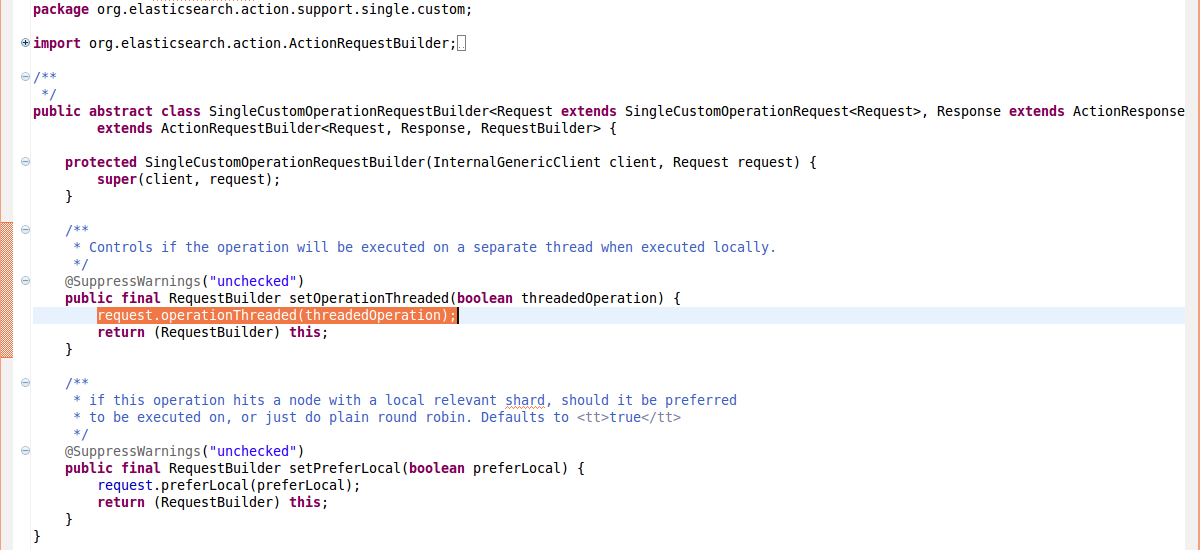
\includegraphics[width=\textwidth]{codingspectator-extract-method-selection.png}
%
\caption{\label{FigCodingSpectatorExtractMethodSelectionExample}A programmer
selects a piece of code to extract into a new method. The selected code is part
of class \texttt{SingleCustomOperationRequestBuilder} from commit
\texttt{bdb1992} of the open-source Elasticsearch project
(\texttt{https://github.com/elasticsearch/elasticsearch}).}
%
\end{figure}

\begin{figure}
%
\centering
%
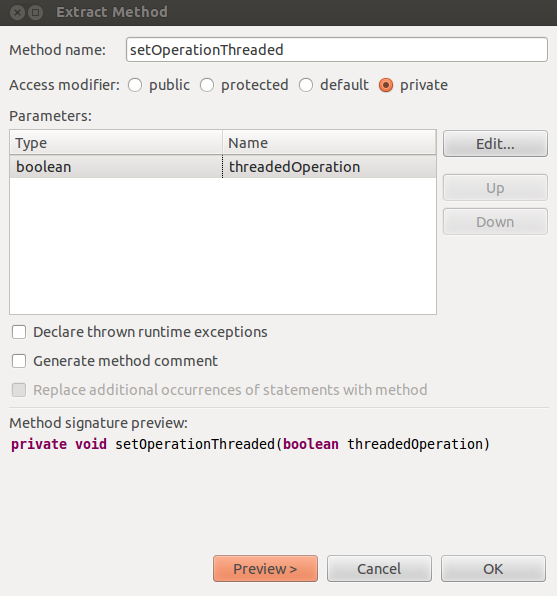
\includegraphics[width=0.5\textwidth]{codingspectator-extract-method-configuration.png}
%
\caption{\label{FigCodingSpectatorExtractMethodConfigurationExample}A programmer
configures an automated Extract Method refactoring by entering the desired name
of the new method.}
%
\end{figure}

\begin{figure}
%
\centering
%
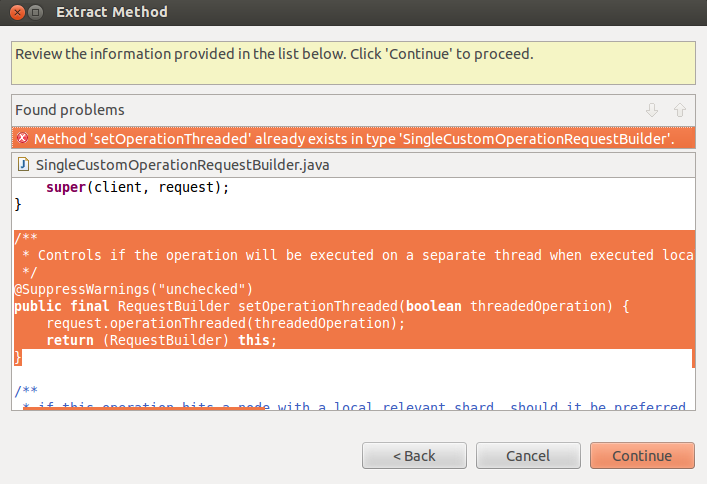
\includegraphics[width=0.6\textwidth]{codingspectator-extract-method-error.png}
%
\caption{\label{FigCodingSpectatorExtractMethodErrorExample}The Extract Method
refactoring reports a name conflict problem to the programmer. The programmer
can either ignore the problem and continue the refactoring, go back to the
configuration page to provide a different name, or cancel the refactoring.}
%
\end{figure}

\begin{figure}
%
\centering
%
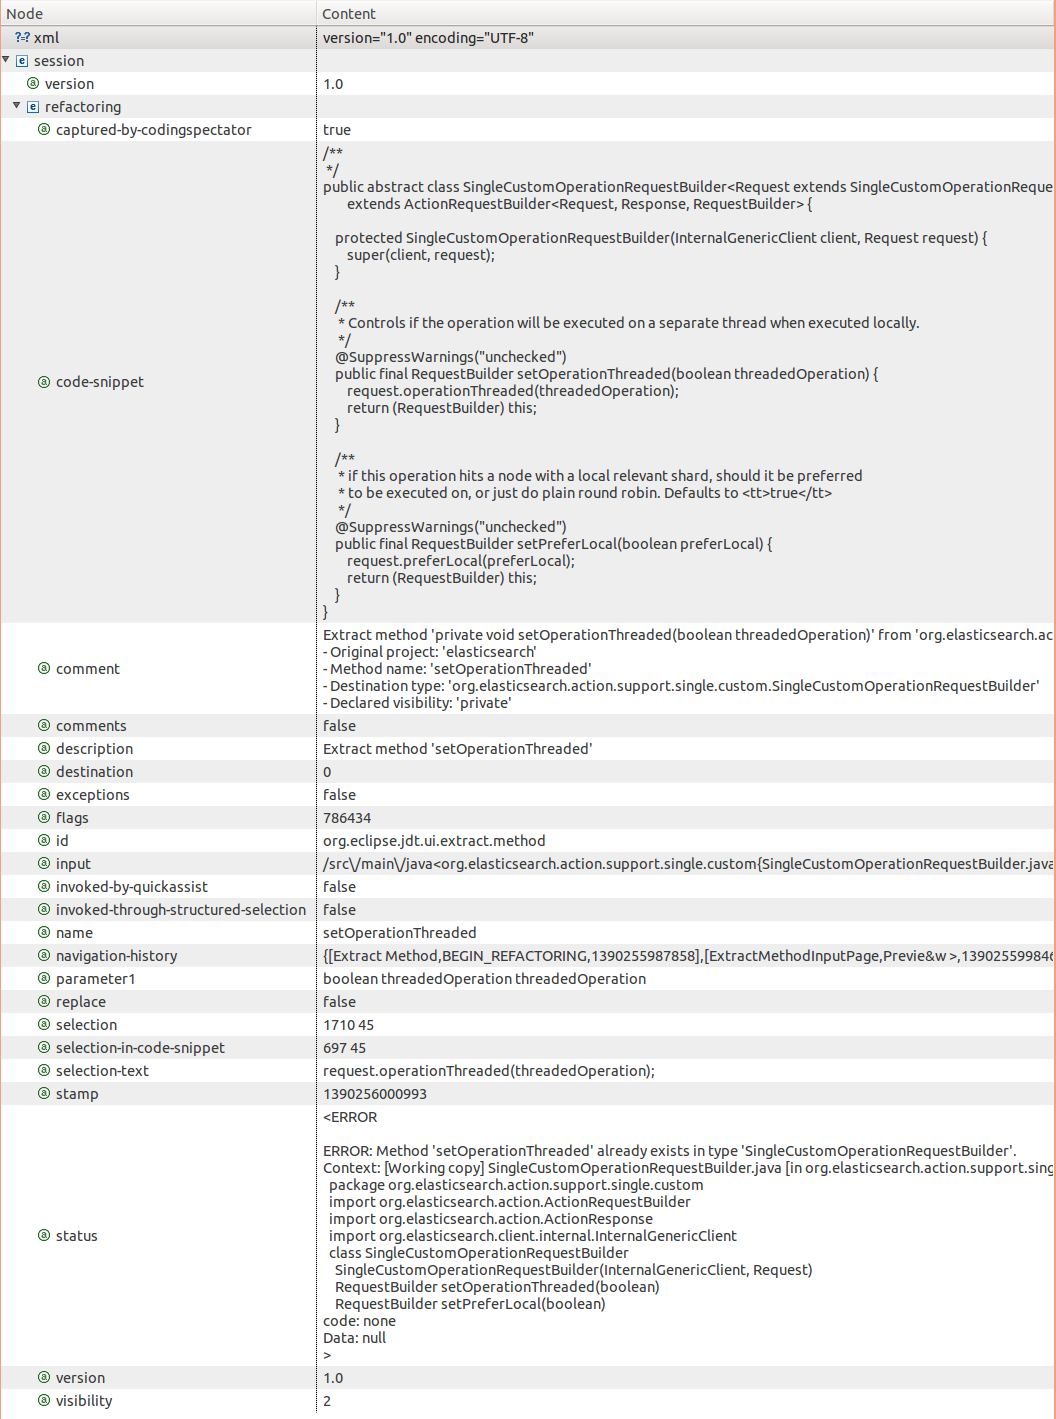
\includegraphics[width=\textwidth]{codingspectator-refactoring-xml.png}
%
\caption{\label{FigCodingSpectatorDescriptorExample}An example refactoring
descriptor recorded by \CodingSpectator.}
%
\end{figure}

\subsubsection{Deploying \CodingSpectator}

Deploying \CodingSpectator{} consists of two main steps:
%
\begin{inparaenum}[(1)]
%
\item setting up a Subversion repository and
%
\item setting up an Eclipse update site.
%
\end{inparaenum}

\paragraph{Setting Up a Subversion Repository}

\CodingSpectator{} regularly submits users' data to a central Subversion
repository. To collect \CodingSpectator's data automatically, you need to set up
a Subversion repository and create accounts for your users. To allow the users
to submit their data to the Subversion repository, you should grant them
appropriate write accesses to the repository.

Using a Version Control System such as Subversion as the data repository has
several advantages:

\begin{enumerate}
%
\item Subversion makes all revisions of each file easily accessible. This makes
  troubleshooting easier for researchers.
%
\item For textual files, Subversion submits only the \emph{changes} made to the
  files as opposed to the entire new file. This differential data submission
  leads to faster submissions.
%
\item There are libraries such as SVNKit\footnote{http://svnkit.com/} that
  provide an API for Subversion operations such as add, update, remove, and
  commit. \CodingSpectator{} uses SVNKit for submitting users' data to the
  central repository.
%
\item Setting up a Subversion server is a well-documented process. This avoids
  the burden of setting up a specialized server.
%
\end{enumerate}

On the other hand, a disadvantage of using Subversion as the data repository is
that it requires the users to maintain a copy of their data on their file
systems. The Subversion working copy on the users' systems takes \emph{space}
and can also cause \emph{merge conflicts}, \eg, if a user restores the contents
of the file system to an earlier version. To handle merge conflicts,
\CodingSpectator{} has built-in support for automatic conflict detection and
resolution. When \CodingSpectator{} detects a merge conflict, it removes the
user's data from the central repository and then submits the new data. Despite
removing the data from the central repository, the researchers can still locate
the merge conflicts and restore the data that was collected before the conflicts occurred.

\CodingSpectator{} prompts the users for their Subversion user names and
passwords when \CodingSpectator{} is about to submit their data.
\CodingSpectator{} gives the users the option to save their passwords in Eclipse
securely. See \url{http://codingspectator.cs.illinois.edu/documentation} for
more information about the features of \CodingSpectator{} for users.

\paragraph{Setting Up an Eclipse Update Site}

Users of \CodingSpectator{} install it from an Eclipse update
site\footnote{\url{http://codingspectator.cs.illinois.edu/installation}}. An
Eclipse update site is an online repository of the JAR and configuration files
that Eclipse requires for installing a plug-in.

You will have to customize \CodingSpectator{} at least by specifying the URL of
the Subversion repository to which \CodingSpectator{} should submit users' data.
You may also want to customize the message that \CodingSpectator{} shows to the
users when it prompts them for their Subversion credentials. You can customize
these aspects of \CodingSpectator{} by changing the configuration files that are
packed in the existing JAR files hosted at the Eclipse update site of
\CodingSpectator. If you need to customize \CodingSpectator{} in more complex
ways that involve changes to its source code, you should follow the instructions
for building \CodingSpectator's update site from source code.

\subsubsection{Extending \CodingSpectator}

In addition to collecting detailed refactoring data, \CodingSpectator{} provides
a reusable infrastructure for collecting Eclipse usage data. Extending
\CodingSpectator{} frees researchers from having to develop many features from
scratch, \eg, Subversion communications, automatic merge conflict detection and
resolution, secure storage of Subversion credentials, and periodic update
reminders.

\CodingSpectator{} provides an Eclipse extension point (id =
\texttt{edu.\-illinois.\-codingspectator.\-monitor.\-core.\-submitter}) and the
following interface:

\begin{lstlisting}
public interface SubmitterListener {
  // hook before svn add
  void preSubmit();
  // hook after svn add and before svn commit
  void preCommit();
  // hook after svn commit
  void postSubmit(boolean succeeded);
}
\end{lstlisting}

The above interface provides three hooks to \CodingSpectator's submission
process. \CodingSpectator{} checks out the Subversion repository into a folder,
which we refer to as the \emph{watched folder}. Then, it executes the Subversion
commands (\eg, add and commit) on the watched folder. A plug-in that extends the
\Code{submitter} extension point and implements the \Code{SubmitterListener}
interface can perform actions before or after two of the Subversion commands that
\CodingSpectator{} executes: add and commit.
%
For example, \CodingSpectator{} overrides the method \Code{preSubmit} to copy
the recorded refactoring descriptors to the watched folder. As another example,
the developers of \CodingSpectator{} made the Eclipse UDC plug-in use the
\Code{submitter} extension point and copy the UDC data to the watched folder. As
a result, \CodingSpectator{} submits the UDC data to the Subversion repository.
Effectively, this is an alternative method to the one presented in
\SecRef{SecUDCHowToUseIt} for collecting UDC data in a central repository.

%TODO: The paragraph above feels like a wrapup partiularly the last sentence.  Can you craft one more sentence with final words of advice to those who want to use Coding Spectator for their research?
% LocalWords: CodingSpectator Urbana Champaign IDE timestamp
%
% LocalWords: CodingTracker refactoring refactorings refactoring's
%
% LocalWords: SVNKit URL usernames online API



\subsection{Existing Data}

Existing UDC data is available through the Eclipse foundation at this URL:
\url{http://archive.eclipse.org/projects/usagedata/}
%could provide more analysis, maybe even BigData

\subsection{Exercises}

\begin{ExerciseList}
 \Exercise[type={long}, difficulty={0}]Define GQM? 
  \Answer Goal-Question-Metric is a methodology for refining a level goal into specific metrics to generate from data
 \Exercise[ type={long}, difficulty={1}]How is GQM Relevant to usage data collection? 
  \Answer It helps the researcher to identify a more specific set of IDE commands useful to their research so they do not have to track all commands in the IDE.
  \Exercise[ type={long}, difficulty={2}]Take an idea for usage monitoring and define a GQM for your idea. 
  \Answer Open-ended question asking students to apply the GQM method to their work.  Check to see that Goals are appropriate goal statements, questions refine the goal and lead the reader towards a specific measureable entity, and metrics are defined with all appropriate dimensions (such as time, and scale).
  \Exercise[ type={long}, difficulty={2}]Using your GQM, identify the usage data attributes you need to collect. 
  \Answer Open-ended question deriving a set of usage data elements from the student's defined GQM.  Usage data atrributes should consist of specific IDE commands, user actions within the editor, or another element measurable with soruce code and IDE access. 

\end{ExerciseList}


\subsection{Eclipse Mylyn Monitor}
